\chapter{Military \& Covert Communications}
\label{ch:military-covert}

\begin{nontechnical}
\textbf{Military communications are like having a secret conversation in a hostile environment}---you need to avoid being jammed, intercepted, or detected while staying connected.

\textbf{Key challenges:}
\begin{itemize}
\item \textbf{Anti-jamming (AJ):} Someone is trying to drown out your signal with noise
\item \textbf{Low probability of intercept (LPI):} Enemies can detect but not decode your message
\item \textbf{Low probability of detection (LPD):} Enemies don't even know you're transmitting
\item \textbf{Secure transmission (TRANSEC):} Even if intercepted, the message is protected
\end{itemize}

\textbf{Real-world examples:}
\begin{itemize}
\item GPS M-code: Military GPS that works even when jammed
\item MILSTAR satellites: Frequency-hopping communications that can't be followed
\item Phased-array radar: Electronic beam steering that's hard to detect
\item Link 16: Tactical data exchange between aircraft, ships, and ground stations
\end{itemize}

\textbf{Core principle:} Spread your signal so thin it's weaker than noise, but use special codes so your receiver can still hear you perfectly. It's like whispering a secret across a crowded room---only someone with the pattern can collect all the pieces.
\end{nontechnical}

\section{Overview}

Military communications systems prioritize \textbf{anti-jamming (AJ)}, \textbf{low probability of intercept (LPI)}, \textbf{low probability of detection (LPD)}, and \textbf{secure transmission (TRANSEC)} over commercial metrics like spectral efficiency. This chapter covers advanced techniques used in GPS M-code, SATCOM FHSS, phased-array radar, Link 16, and covert communications.

\begin{keyconcept}
The fundamental principle enabling military communications is \textbf{processing gain} from spread spectrum modulation. By spreading the signal across a bandwidth much wider than necessary, the power spectral density drops below the noise floor, providing LPI/LPD characteristics while simultaneously enabling anti-jamming through despreading gain.
\end{keyconcept}

Before diving into the technical details, here are the core concepts explained in everyday terms:

\subsubsection{Why Military Communications Are
Different}\label{why-military-communications-are-different}

\textbf{Imagine trying to have a conversation in a crowded, hostile
room} where: - Someone is shouting over you (jamming) - Others are
listening to steal your secrets (interception) - You need to talk
without being noticed (covert)

Military communications solve these problems in ways regular WiFi or
cell phones don\textquotesingle t need to.

\begin{center}\rule{0.5\linewidth}{0.5pt}\end{center}

\subsubsection{The ``Whisper in the Crowd''
Analogy}\label{the-whisper-in-the-crowd-analogy}

\textbf{Spread Spectrum} = Speaking very quietly across a huge room

Instead of shouting one clear message, you: 1. \textbf{Whisper
fragments} of your message to many places at once 2. \textbf{Spread it
so thin} that each piece sounds like background noise 3. \textbf{Only
someone with the secret pattern} can collect all the pieces and
understand you

\textbf{Real-world result}: Your signal is literally \textbf{weaker than
background noise}, yet your intended receiver hears it perfectly.
Enemies just hear static.

\textbf{Example}: GPS M-code is 20 times weaker than the noise floor,
yet your military GPS receiver locks on instantly. A
spy\textquotesingle s receiver? Just noise.

\begin{center}\rule{0.5\linewidth}{0.5pt}\end{center}

\subsubsection{The ``Concert Hall Spotlight''
Analogy}\label{the-concert-hall-spotlight-analogy}

\textbf{Phased-Array Antennas (AESA)} = Pointing a beam of radio energy

Think of a traditional dish antenna like a flashlight-\/-\/-it points
one direction, and moving it takes time.

\textbf{AESA is like a concert hall\textquotesingle s lighting system}:
- \textbf{Hundreds of tiny lights} (antenna elements) -
\textbf{Computer-controlled} to turn on/off in precise patterns -
\textbf{Creates a ``spotlight''} that can instantly jump to different
parts of the room - \textbf{Multiple spotlights} can exist
simultaneously (track many targets)

\textbf{Real-world result}: F-22 radar can track 100 aircraft, jam enemy
radars, and guide missiles-\/-\/-all at once, all electronically, no
moving parts.

\begin{center}\rule{0.5\linewidth}{0.5pt}\end{center}

\subsubsection{The ``Secret Handshake''
Analogy}\label{the-secret-handshake-analogy}

\textbf{Frequency Hopping} = Changing radio channels thousands of times
per second

Imagine a conversation where: 1. You and your friend \textbf{agree on a
secret pattern} of which channel to use when 2. Every millisecond, you
both \textbf{jump to a new frequency} following the pattern 3.
\textbf{Enemies can\textquotesingle t follow} because they
don\textquotesingle t know the pattern 4. Even if they jam one
frequency, you\textquotesingle re already gone

\textbf{Real-world result}: Military satellite phones (MILSTAR) hop
1000+ times per second across a gigahertz of spectrum. A jammer would
need to jam the entire band with megawatts of power-\/-\/-impractical.

\begin{center}\rule{0.5\linewidth}{0.5pt}\end{center}

\subsubsection{The ``Invisible Ink''
Analogy}\label{the-invisible-ink-analogy}

\textbf{Low Probability of Detection (LPD)} = Radio signals that
don\textquotesingle t look like signals

Imagine hiding a message by: 1. \textbf{Writing each letter} on a
separate grain of sand 2. \textbf{Scattering the sand} across a beach 3.
\textbf{Only the recipient} knows which grains to collect

\textbf{Real-world result}: Covert radios transmit at power levels
1000\$\textbackslash times\$ below what receivers normally detect. Even
sensitive spy equipment can\textquotesingle t tell the difference
between the transmission and natural radio noise.

\begin{center}\rule{0.5\linewidth}{0.5pt}\end{center}

\subsubsection{The ``Smart Echo'' Analogy}\label{the-smart-echo-analogy}

\textbf{Anti-Jamming (AJ)} = Fighting back against interference

When an enemy tries to jam your signal: 1. \textbf{Your antenna
``learns''} where the jammer is located 2. \textbf{Creates a ``null''}
(deaf spot) pointing at the jammer 3. \textbf{Amplifies signals} from
your intended direction

Think of it like \textbf{noise-canceling headphones for
radio}-\/-\/-specifically canceling out the jammer while hearing your
friend.

\textbf{Real-world result}: GPS receivers with anti-jam antennas (CRPA)
can reject jammers that are 10,000\$\textbackslash times\$ stronger than
the GPS satellite signal.

\begin{center}\rule{0.5\linewidth}{0.5pt}\end{center}

\subsubsection{Key Concepts Simplified}\label{key-concepts-simplified}

{\def\LTcaptype{} % do not increment counter
\begin{longtable}[]{@{}
  >{\raggedright\arraybackslash}p{(\linewidth - 4\tabcolsep) * \real{0.2000}}
  >{\raggedright\arraybackslash}p{(\linewidth - 4\tabcolsep) * \real{0.4000}}
  >{\raggedright\arraybackslash}p{(\linewidth - 4\tabcolsep) * \real{0.4000}}@{}}
\toprule\noalign{}
\begin{minipage}[b]{\linewidth}\raggedright
Concept
\end{minipage} & \begin{minipage}[b]{\linewidth}\raggedright
Everyday Analogy
\end{minipage} & \begin{minipage}[b]{\linewidth}\raggedright
Military Benefit
\end{minipage} \\
\midrule\noalign{}
\endhead
\bottomrule\noalign{}
\endlastfoot
\textbf{Spread Spectrum} & Whisper spread across a huge room & Signal
hidden below noise floor \\
\textbf{Processing Gain} & Collecting 1000 whispers back into speech &
Overcomes jammers and noise \\
\textbf{Frequency Hopping} & Changing channels
1000\$\textbackslash times\$ per second & Enemy can\textquotesingle t
follow or jam \\
\textbf{Phased Array} & Computer-controlled spotlight & Instant beam
steering, multi-target \\
\textbf{Encryption} & Secret language only you and friend know & Even
intercepted messages are useless \\
\textbf{Beamforming} & Talking through a directional megaphone & Only
intended receiver hears you \\
\end{longtable}
}

\begin{center}\rule{0.5\linewidth}{0.5pt}\end{center}

\subsubsection{Why This Matters for
Chimera}\label{why-this-matters-for-chimera}

Chimera helps you \textbf{visualize and experiment} with these concepts:
- \textbf{Build spread spectrum systems} in your browser - \textbf{See
jamming resistance} in real-time plots - \textbf{Experiment with
frequency hopping} patterns - \textbf{Understand phased arrays} through
interactive simulations

\textbf{You don\textquotesingle t need a million-dollar
lab}-\/-\/-Chimera brings military-grade DSP concepts to anyone with
curiosity and a web browser.

\begin{center}\rule{0.5\linewidth}{0.5pt}\end{center}

\subsubsection{What You\textquotesingle ll Learn in This
Document}\label{what-youll-learn-in-this-document}

The sections below explain \textbf{how these systems actually work}: -
\textbf{SATCOM Frequency Hopping}: How military satellites resist
jamming - \textbf{GPS M-Code}: Why military GPS works when civilian GPS
is jammed - \textbf{Phased-Array Radar}: How F-22s and destroyers
``see'' electronically - \textbf{Link 16}: The tactical data network
connecting planes, ships, and missiles - \textbf{Covert Communications}:
How to transmit data invisibly

\textbf{If you\textquotesingle re new to DSP}: Start with
{[}{[}Spread-Spectrum-(DSSS-FHSS){]}{]} for foundational concepts, then
return here.

\textbf{If you\textquotesingle re experienced}: Skip to the technical
sections-\/-\/-detailed math, code examples, and real-world system specs
await.

\section{Mathematical Description}

\subsection{Processing Gain}

The fundamental enabler of military communications is \textbf{processing gain}, which relates the spread bandwidth to the information bandwidth:
\begin{equation}
G = \frac{B_{\text{spread}}}{B_{\text{info}}} = \frac{R_{\text{chip}}}{R_{\text{bit}}}
\label{eq:processing-gain}
\end{equation}
where:
\begin{itemize}
\item $G$ = processing gain (dimensionless, often expressed in dB: $G_{\text{dB}} = 10\log_{10}(G)$)
\item $B_{\text{spread}}$ = spread bandwidth (Hz)
\item $B_{\text{info}}$ = information bandwidth (Hz)
\item $R_{\text{chip}}$ = chip rate (chips/second)
\item $R_{\text{bit}}$ = bit rate (bits/second)
\end{itemize}

\subsection{Power Spectral Density Reduction}

Spreading the signal reduces its power spectral density (PSD), making it harder to detect:
\begin{equation}
\text{PSD}_{\text{spread}} = \frac{P_{\text{TX}}}{B_{\text{spread}}}
\label{eq:psd-spread}
\end{equation}
where:
\begin{itemize}
\item $\text{PSD}_{\text{spread}}$ = power spectral density of spread signal (W/Hz)
\item $P_{\text{TX}}$ = total transmit power (W)
\end{itemize}

For LPD operation, the PSD must be below the thermal noise floor:
\begin{equation}
\text{PSD}_{\text{spread}} < N_0 = k_B T
\label{eq:lpd-condition}
\end{equation}
where:
\begin{itemize}
\item $N_0$ = thermal noise power spectral density (W/Hz)
\item $k_B = 1.38 \times 10^{-23}$ J/K = Boltzmann's constant
\item $T$ = system noise temperature (K), typically $T \approx 290$ K (room temperature)
\end{itemize}

\subsection{Jamming Margin}

The ability of a spread spectrum system to resist jamming is quantified by the jamming margin:
\begin{equation}
M_J = G_{\text{dB}} - \left(\frac{J}{S}\right)_{\text{dB}} - \left(\frac{E_b}{N_0}\right)_{\text{req}} - L_{\text{impl}}
\label{eq:jamming-margin}
\end{equation}
where:
\begin{itemize}
\item $M_J$ = jamming margin (dB); positive value indicates link survives
\item $G_{\text{dB}}$ = processing gain (dB)
\item $(J/S)_{\text{dB}}$ = jammer-to-signal power ratio at receiver (dB)
\item $(E_b/N_0)_{\text{req}}$ = required energy per bit to noise ratio for target BER (dB)
\item $L_{\text{impl}}$ = implementation losses (dB), typically 2-3 dB
\end{itemize}

\subsection{Direct Sequence Spread Spectrum (DSSS)}

In DSSS, each data bit is multiplied by a high-rate pseudo-random code:
\begin{equation}
s_{\text{DSSS}}(t) = A \cdot d(t) \cdot c(t) \cdot \cos(2\pi f_c t)
\label{eq:dsss-signal}
\end{equation}
where:
\begin{itemize}
\item $A$ = carrier amplitude
\item $d(t)$ = data sequence ($\pm 1$)
\item $c(t)$ = spreading code sequence ($\pm 1$), chip rate $R_{\text{chip}} \gg R_{\text{bit}}$
\item $f_c$ = carrier frequency (Hz)
\end{itemize}

The receiver despreads by multiplying with a synchronized replica of $c(t)$:
\begin{equation}
r(t) \cdot c(t) = [s_{\text{DSSS}}(t) + n(t) + j(t)] \cdot c(t)
\label{eq:dsss-despread}
\end{equation}
where:
\begin{itemize}
\item $n(t)$ = additive white Gaussian noise
\item $j(t)$ = jammer signal
\end{itemize}

Since $c(t) \cdot c(t) = 1$ (code autocorrelation), the desired signal is recovered while noise and jamming remain spread.

\subsection{Frequency Hopping Spread Spectrum (FHSS)}

In FHSS, the carrier frequency hops pseudo-randomly across a set of channels:
\begin{equation}
s_{\text{FHSS}}(t) = A \cdot d(t) \cdot \cos(2\pi f_i(t) t)
\label{eq:fhss-signal}
\end{equation}
where:
\begin{itemize}
\item $f_i(t)$ = time-varying carrier frequency, $i \in \{1, 2, \ldots, N_{\text{hop}}\}$
\item $N_{\text{hop}}$ = number of frequency channels in hop set
\end{itemize}

The processing gain for FHSS is:
\begin{equation}
G_{\text{FHSS}} = N_{\text{hop}}
\label{eq:fhss-gain}
\end{equation}

The hop dwell time is:
\begin{equation}
T_{\text{dwell}} = \frac{1}{R_{\text{hop}}}
\label{eq:hop-dwell}
\end{equation}
where:
\begin{itemize}
\item $T_{\text{dwell}}$ = time spent on each frequency (s)
\item $R_{\text{hop}}$ = hop rate (hops/second)
\end{itemize}

\subsection{Phased Array Beamforming}

A phased array antenna with $N$ elements steers its beam by applying progressive phase shifts:
\begin{equation}
\phi_n = \frac{2\pi d}{\lambda} n \sin(\theta)
\label{eq:phase-shift}
\end{equation}
where:
\begin{itemize}
\item $\phi_n$ = phase shift for element $n$ (radians)
\item $d$ = element spacing (m)
\item $\lambda$ = wavelength (m)
\item $\theta$ = desired beam angle from array normal (degrees)
\item $n$ = element index, $n \in \{0, 1, \ldots, N-1\}$
\end{itemize}

The array gain is:
\begin{equation}
G_{\text{array}} = N \cdot G_{\text{element}}
\label{eq:array-gain}
\end{equation}
where:
\begin{itemize}
\item $G_{\text{array}}$ = total array gain (linear)
\item $G_{\text{element}}$ = gain of individual element (linear)
\end{itemize}

In dB:
\begin{equation}
G_{\text{array, dB}} = 10\log_{10}(N) + G_{\text{element, dBi}}
\label{eq:array-gain-db}
\end{equation}

\subsection{The LPI/LPD/AJ Triad}

\textbf{1. Low Probability of Intercept (LPI):} Enemy can detect transmission but cannot decode it.

\textbf{Techniques:}
\begin{itemize}
\item Spread spectrum (DSSS/FHSS)---signal below noise floor
\item Directional antennas---narrow beamwidths
\item Burst transmissions---short dwell time
\item Encryption---content secure even if intercepted
\end{itemize}

\textbf{2. Low Probability of Detection (LPD):} Enemy cannot detect that transmission is occurring.

\textbf{Techniques:}
\begin{itemize}
\item Ultra-wideband spread spectrum ($G > 30$ dB)
\item Frequency diversity---avoid surveillance bands
\item Power management---minimal radiated power
\item Emission control (EMCON)---radio silence protocols
\end{itemize}

\textbf{3. Anti-Jamming (AJ):} Maintain link under deliberate enemy interference.

\textbf{Techniques:}
\begin{itemize}
\item Processing gain---overcomes jammer power
\item Nulling antennas---reject jammer direction
\item Frequency hopping---avoid narrowband jamming
\item Adaptive filters---real-time interference cancellation
\end{itemize}

\begin{calloutbox}{Relationship Between LPI/LPD/AJ}
All three capabilities are enabled by processing gain $G$. Higher $G$ results in lower PSD, making signals harder to detect (LPD), intercept (LPI), and jam (AJ). The key trade-off is bandwidth: achieving high $G$ requires wide bandwidth, which may not always be available in congested spectrum.
\end{calloutbox}

\section{Modulation and Demodulation}

\subsection{DSSS Transmitter and Receiver}

\textbf{DSSS Transmitter:}

\begin{center}
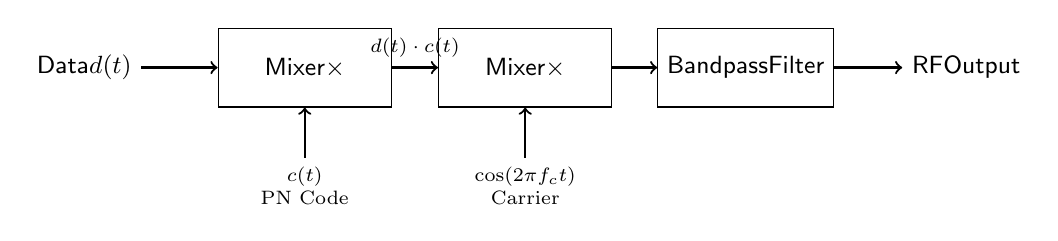
\begin{tikzpicture}[
  block/.style={rectangle, draw, minimum width=2.2cm, minimum height=1cm, font=\sffamily\small},
  node distance=2.5cm,
  font=\small
]
\node (input) {\sffamily Data\\$d(t)$};
\node[block, right of=input, node distance=2.8cm] (mult1) {Mixer\\$\times$};
\node[block, right of=mult1, node distance=2.8cm] (mult2) {Mixer\\$\times$};
\node[block, right of=mult2, node distance=2.8cm] (bpf) {Bandpass\\Filter};
\node[right of=bpf, node distance=2.8cm] (output) {\sffamily RF\\Output};

\node[below of=mult1, node distance=1.5cm, font=\scriptsize, align=center] (code) {$c(t)$\\PN Code};
\node[below of=mult2, node distance=1.5cm, font=\scriptsize, align=center] (carrier) {$\cos(2\pi f_c t)$\\Carrier};

\draw[->,thick] (input) -- (mult1);
\draw[->,thick] (code) -- (mult1);
\draw[->,thick] (mult1) -- node[above,font=\scriptsize] {$d(t) \cdot c(t)$} (mult2);
\draw[->,thick] (carrier) -- (mult2);
\draw[->,thick] (mult2) -- (bpf);
\draw[->,thick] (bpf) -- (output);
\end{tikzpicture}
\end{center}

\textbf{Process:}
\begin{enumerate}
\item \textbf{Spreading:} Multiply data $d(t)$ by high-rate PN code $c(t)$
\item \textbf{Upconversion:} Multiply by carrier to shift to RF frequency
\item \textbf{Filtering:} Bandpass filter removes out-of-band emissions
\end{enumerate}

\textbf{DSSS Receiver:}

\begin{center}
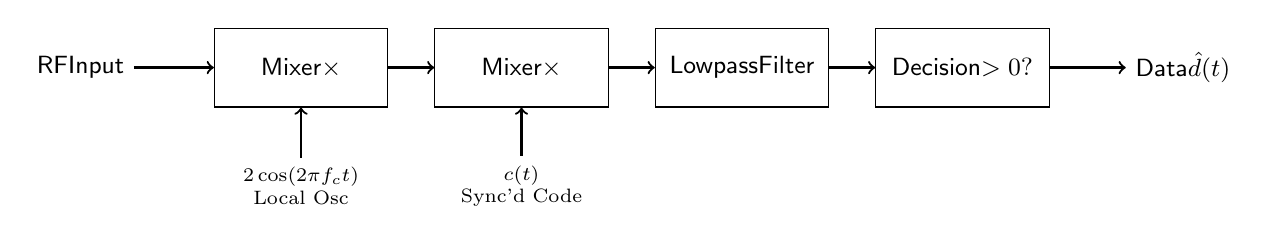
\begin{tikzpicture}[
  block/.style={rectangle, draw, minimum width=2.2cm, minimum height=1cm, font=\sffamily\small},
  node distance=2.5cm,
  font=\small
]
\node (input) {\sffamily RF\\Input};
\node[block, right of=input, node distance=2.8cm] (mult1) {Mixer\\$\times$};
\node[block, right of=mult1, node distance=2.8cm] (mult2) {Mixer\\$\times$};
\node[block, right of=mult2, node distance=2.8cm] (lpf) {Lowpass\\Filter};
\node[block, right of=lpf, node distance=2.8cm] (decide) {Decision\\$>0?$};
\node[right of=decide, node distance=2.8cm] (output) {\sffamily Data\\$\hat{d}(t)$};

\node[below of=mult1, node distance=1.5cm, font=\scriptsize, align=center] (carrier2) {$2\cos(2\pi f_c t)$\\Local Osc};
\node[below of=mult2, node distance=1.5cm, font=\scriptsize, align=center] (code2) {$c(t)$\\Sync'd Code};

\draw[->,thick] (input) -- (mult1);
\draw[->,thick] (carrier2) -- (mult1);
\draw[->,thick] (mult1) -- (mult2);
\draw[->,thick] (code2) -- (mult2);
\draw[->,thick] (mult2) -- (lpf);
\draw[->,thick] (lpf) -- (decide);
\draw[->,thick] (decide) -- (output);
\end{tikzpicture}
\end{center}

\textbf{Process:}
\begin{enumerate}
\item \textbf{Downconversion:} Multiply by local oscillator to baseband
\item \textbf{Despreading:} Multiply by synchronized PN code replica
\item \textbf{Integration:} Lowpass filter accumulates signal energy
\item \textbf{Decision:} Threshold detector recovers data bits
\end{enumerate}

\begin{warningbox}
\textbf{Code synchronization is critical.} The receiver's PN code must be aligned to within a fraction of a chip period. This requires acquisition (coarse alignment) and tracking (fine alignment) subsystems. Loss of synchronization results in complete signal loss, as the despreading process fails.
\end{warningbox}

\subsection{FHSS Frequency Hopping Pattern}

\textbf{Frequency Hopping Visualization:}

\begin{center}
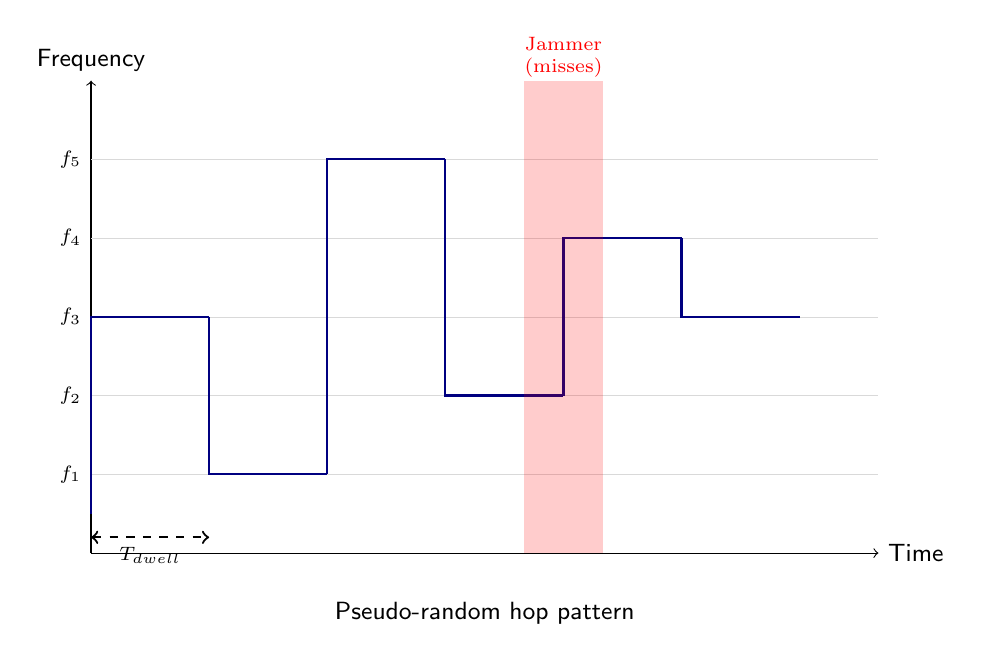
\begin{tikzpicture}[scale=1.0]
% Axes
\draw[->] (0,0) -- (10,0) node[right,font=\sffamily\small] {Time};
\draw[->] (0,0) -- (0,6) node[above,font=\sffamily\small] {Frequency};

% Frequency channels
\foreach \y in {1,2,3,4,5} {
  \draw[very thin,gray!30] (0,\y) -- (10,\y);
  \node[left,font=\scriptsize] at (0,\y) {$f_{\y}$};
}

% Hop pattern
\draw[thick,NavyBlue] (0,0.5) -- (0,3) -- (1.5,3);
\draw[thick,NavyBlue] (1.5,3) -- (1.5,1) -- (3,1);
\draw[thick,NavyBlue] (3,1) -- (3,5) -- (4.5,5);
\draw[thick,NavyBlue] (4.5,5) -- (4.5,2) -- (6,2);
\draw[thick,NavyBlue] (6,2) -- (6,4) -- (7.5,4);
\draw[thick,NavyBlue] (7.5,4) -- (7.5,3) -- (9,3);

% Dwell time annotation
\draw[<->,thick,dashed] (0,0.2) -- (1.5,0.2) node[midway,below,font=\scriptsize] {$T_{\text{dwell}}$};

% Jammer
\fill[red,opacity=0.2] (5.5,0) rectangle (6.5,6);
\node[red,font=\scriptsize,align=center] at (6,6.3) {Jammer\\(misses)};

\node[below,font=\sffamily\small] at (5,-0.5) {Pseudo-random hop pattern};
\end{tikzpicture}
\end{center}

\textbf{Key features:}
\begin{itemize}
\item Each hop dwells for time $T_{\text{dwell}} = 1/R_{\text{hop}}$
\item Hop pattern is pseudo-random, determined by cryptographic key
\item Jammer cannot predict next frequency---must jam entire band
\item Fast hopping ($T_{\text{dwell}} < 100$ µs) defeats follower jammers
\end{itemize}

\subsection{Phased Array Beam Steering}

\textbf{Electronic Beamforming Principle:}

\begin{center}
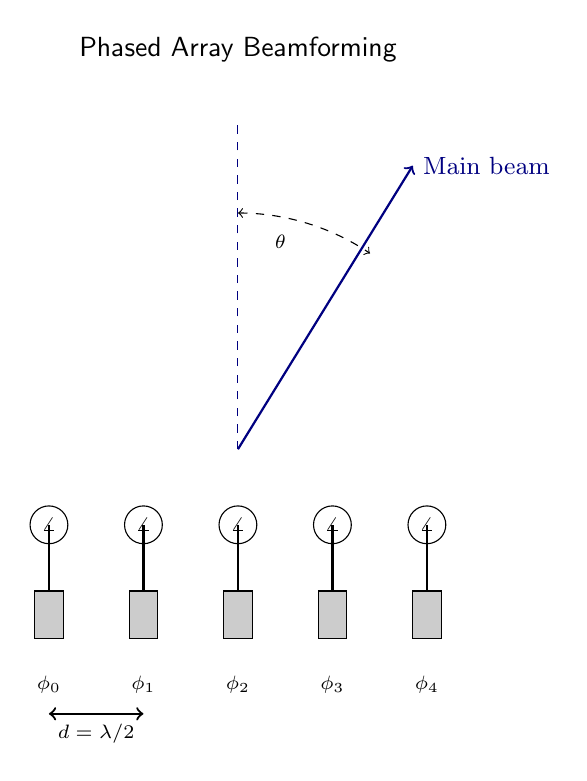
\begin{tikzpicture}[scale=1.2]
% Array elements
\foreach \x in {0,1,2,3,4} {
  \draw[fill=black!20] (\x,0) rectangle (\x+0.3,0.5);
  \node[below,font=\scriptsize] at (\x+0.15,-0.3) {$\phi_{\x}$};
}

% Phase shifters
\foreach \x in {0,1,2,3,4} {
  \draw[thick] (\x+0.15,0.5) -- (\x+0.15,1.2);
  \draw (\x+0.15,1.2) circle (0.2);
  \node[font=\tiny] at (\x+0.15,1.2) {$\angle$};
}

% Beam pattern (main lobe)
\draw[thick,NavyBlue,->] (2.15,2) -- (4,5) node[right,font=\small] {Main beam};
\draw[dashed,NavyBlue] (2.15,2) -- (2.15,5.5);

% Angle annotation
\draw[<->,dashed] (2.15,4.5) arc (90:56:2.5);
\node[font=\scriptsize] at (2.6,4.2) {$\theta$};

% Element spacing
\draw[<->,thick] (0.15,-0.8) -- (1.15,-0.8) node[midway,below,font=\scriptsize] {$d = \lambda/2$};

% Title
\node[above,font=\sffamily] at (2.15,6) {Phased Array Beamforming};
\end{tikzpicture}
\end{center}

\textbf{Beam steering equation:}
\begin{itemize}
\item Progressive phase shift: $\phi_n = (2\pi d/\lambda) n \sin(\theta)$
\item Beam angle $\theta$ controlled electronically (no mechanical motion)
\item Switching time: $<$ 1 µs (vs. seconds for mechanical scanning)
\item Multiple beams possible simultaneously (multi-target tracking)
\end{itemize}

\section{Applications}

\subsection{SATCOM Frequency Hopping (FHSS)}

Military satellite communications use FHSS for TRANSEC (transmission
security).

\subsubsection{X-Band MILSTAR/MUOS
Systems}\label{x-band-milstarmuos-systems}

\textbf{MILSTAR (Military Strategic and Tactical Relay)}:

\begin{verbatim}
Frequency: X-band uplink (7-8 GHz), Ka-band downlink (20-21 GHz)
Hop rate: 100-1000+ hops/second
Hop set: 1000+ frequencies across 1 GHz bandwidth
Dwell time: <1 ms per hop
Modulation: BPSK, QPSK, 8-PSK (adaptive)
Data rate: 75 bps - 1.544 Mbps (T1)
Satellite constellation: 5 GEO satellites (global coverage)

TRANSEC:
- Hopping pattern: Cryptographically generated (NSA algorithm)
- Synchronization: GPS time + KEK (Key Encryption Key)
- Pattern period: Days to weeks (never repeats observably)
- Anti-spoofing: Authenticated hop sequence
\end{verbatim}

\textbf{LPI/LPD characteristics}:

\begin{verbatim}
Power spectral density (PSD):
PSD = P_TX / BW_hop_set
    = 100 W / 1 GHz
    = 0.1 mW/MHz
     -70 dBm/MHz (at satellite, 40,000 km away)

Compare to thermal noise floor:
Noise = -174 dBm/Hz + 10·log(BW) = -114 dBm/MHz (1 MHz BW)

PSD_signal < Noise  Undetectable to wideband receiver!

Detectability only with:
- Exact hopping pattern (requires key)
- Synchronized receiver (requires network access)
- Correct modulation/demodulation (requires ICD)
\end{verbatim}

\begin{center}\rule{0.5\linewidth}{0.5pt}\end{center}

\textbf{MUOS (Mobile User Objective System)}:

\begin{verbatim}
Frequency: UHF uplink (300-318 MHz), UHF downlink (243-318 MHz)
Waveform: WCDMA (Wideband CDMA) + FHSS hybrid
Hop rate: Classified (estimated >500 hps)
Data rate: Up to 64 kbps voice, 10 Mbps data
Compatibility: Legacy UFO (Ultra High Frequency Follow-On)

Key features:
- Smartphone-like interface for warfighters
- Near-global coverage (5 GEO + legacy satellites)
- Jam-resistant waveform (60+ dB margin)
- Integrated encryption (Type 1 NSA)
\end{verbatim}

\begin{center}\rule{0.5\linewidth}{0.5pt}\end{center}

\subsubsection{FHSS Anti-Jam
Performance}\label{fhss-anti-jam-performance}

\textbf{Processing gain calculation}:

\begin{verbatim}
G(dB) = 10·log(Hop_Set_Size)

Example (MILSTAR):
- Hop set: 1000 frequencies
- G = 10·log(1000) = 30 dB

Jamming margin:
Margin = G - J/S - (Eb/N)_req - Losses

J/S = Jammer power / Signal power (at receiver)

Scenario:
- G = 30 dB
- J/S = 40 dB (jammer 10,000× stronger!)
- (Eb/N)_req = 10 dB (BPSK, BER = 10)
- Losses = 3 dB (implementation)

Margin = 30 - 40 - 10 - 3 = -23 dB  **LINK FAILS**

Countermeasures:
1. Directional antenna: +20 dB gain toward satellite, nulls toward jammer
   Effective J/S = 40 - 20 = 20 dB
   Margin = 30 - 20 - 10 - 3 = -3 dB  **MARGINAL**

2. Error-correction coding: Turbo/LDPC code rate-1/3
   Coding gain: +5 dB
   Margin = -3 + 5 = 2 dB  **LINK SURVIVES**

3. Burst transmission: Transmit 10× faster, listen 90% of time
   Jammer must hit exact burst time  effective J/S reduces by 10 dB
\end{verbatim}

\begin{center}\rule{0.5\linewidth}{0.5pt}\end{center}

\subsubsection{Follower Jamming
Resistance}\label{follower-jamming-resistance}

\textbf{Threat}: Smart jammer detects hop, jams that frequency.

\textbf{Timing analysis}:

\begin{verbatim}
Dwell time: 1 ms (MILSTAR)
Jammer detection: 100 s (fast energy detector)
Frequency switching: 50 s (agile synthesizer)

Total jammer delay: 150 s

Effective jam time: 1 ms - 150 s = 850 s (85% of hop)

Countermeasure: Fast hopping
- Dwell time: 100 s (10× faster)
- Effective jam: 100 - 150 = 0 s (jammer too slow!)

Modern military systems: 10-100 s dwell times
\end{verbatim}

\begin{center}\rule{0.5\linewidth}{0.5pt}\end{center}

\subsection{\texorpdfstring{ GPS M-Code (Military
GPS)}{ GPS M-Code (Military GPS)}}\label{gps-m-code-military-gps}

\textbf{GPS Modernization}: M-code provides jam-resistant, encrypted
positioning for military users.

\subsubsection{Signal Structure}\label{signal-structure}

\textbf{GPS L1 M-Code}:

\begin{verbatim}
Carrier frequency: 1575.42 MHz (L1)
Chip rate: 5.115 Mcps (5× faster than C/A code)
Code length: Classified (estimated ~10^13 chips  never repeats)
Modulation: BOC(10,5) - Binary Offset Carrier
Processing gain: ~50 dB (vs. 43 dB for C/A)
Power: 6.5 dB stronger than C/A code
Security: Encrypted, authenticated (NSA keys)
\end{verbatim}

\textbf{GPS L2 M-Code}:

\begin{verbatim}
Carrier frequency: 1227.60 MHz (L2)
Same structure as L1 M-code
Dual-frequency  ionospheric correction
\end{verbatim}

\begin{center}\rule{0.5\linewidth}{0.5pt}\end{center}

\subsubsection{BOC Modulation}\label{boc-modulation}

\textbf{Binary Offset Carrier (BOC)} modulates the chip sequence with a square wave subcarrier, creating a split-spectrum signature that improves multipath rejection and coexistence with C/A code.

\textbf{BOC(m,n) notation:}
\begin{itemize}
\item $m$ = subcarrier frequency multiplier (MHz)
\item $n$ = chip rate multiplier (MHz)
\end{itemize}

For BOC(10,5):
\begin{equation}
f_{\text{sub}} = 10.23 \text{ MHz} \quad \text{(2$\times$ C/A chip rate)}
\end{equation}
\begin{equation}
R_{\text{chip}} = 5.115 \text{ Mcps} \quad \text{(5$\times$ C/A chip rate)}
\end{equation}

\textbf{BOC Modulation Spectrum:}

\begin{center}
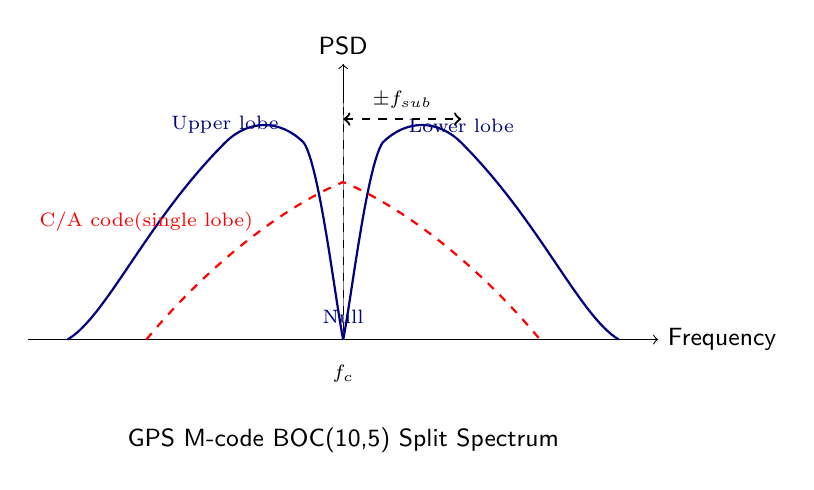
\begin{tikzpicture}[scale=1.0]
% Axes
\draw[->] (-4,0) -- (4,0) node[right,font=\sffamily\small] {Frequency};
\draw[->] (0,0) -- (0,3.5) node[above,font=\sffamily\small] {PSD};

% Center frequency marker
\draw[dashed,gray] (0,0) -- (0,3);
\node[below,font=\scriptsize] at (0,-0.2) {$f_c$};

% BOC split spectrum (two main lobes)
\draw[thick,NavyBlue] (-3.5,0) .. controls (-3,0.3) and (-2.5,1.5) .. (-1.5,2.5) 
  .. controls (-1.2,2.8) and (-0.8,2.8) .. (-0.5,2.5)
  .. controls (-0.3,2.2) and (-0.1,0.5) .. (0,0);
\draw[thick,NavyBlue] (0,0) .. controls (0.1,0.5) and (0.3,2.2) .. (0.5,2.5)
  .. controls (0.8,2.8) and (1.2,2.8) .. (1.5,2.5)
  .. controls (2.5,1.5) and (3,0.3) .. (3.5,0);

% Peak labels
\node[above,font=\scriptsize,NavyBlue] at (-1.5,2.5) {Upper lobe};
\node[above,font=\scriptsize,NavyBlue] at (1.5,2.5) {Lower lobe};

% Frequency offset annotation
\draw[<->,thick,dashed] (0,2.8) -- (1.5,2.8) node[midway,above,font=\scriptsize] {$\pm f_{\text{sub}}$};

% C/A code spectrum (for comparison)
\draw[thick,red,dashed] (-2.5,0) .. controls (-1.5,1.2) and (-0.5,1.8) .. (0,2)
  .. controls (0.5,1.8) and (1.5,1.2) .. (2.5,0);
\node[red,font=\scriptsize] at (-2.5,1.5) {C/A code\\(single lobe)};

% Null at center
\node[below,font=\scriptsize,NavyBlue] at (0,0.5) {Null};

\node[below,font=\sffamily\small] at (0,-1) {GPS M-code BOC(10,5) Split Spectrum};
\end{tikzpicture}
\end{center}

\textbf{BOC signal equation:}
\begin{equation}
s_{\text{BOC}}(t) = \text{sign}[\sin(2\pi f_{\text{sub}} t)] \cdot c(t) \cdot \cos(2\pi f_c t)
\end{equation}
where:
\begin{itemize}
\item $\text{sign}[\cdot]$ = square wave subcarrier ($\pm 1$)
\item $c(t)$ = spreading code
\item $f_c$ = carrier frequency (L1: 1575.42 MHz)
\end{itemize}

\textbf{Advantages of BOC:}
\begin{itemize}
\item Split spectrum reduces interference with C/A code at $f_c$
\item Sharper autocorrelation improves ranging accuracy
\item Higher bandwidth provides multipath rejection
\item Processing gain: $\sim 50$ dB (vs. 43 dB for C/A code)
\end{itemize}

\textbf{Power and Processing Gain:}
\begin{equation}
G_{\text{M-code}} = 10\log_{10}\left(\frac{f_{\text{sub}}}{R_{\text{bit}}}\right) \approx 50 \text{ dB}
\end{equation}
where:
\begin{itemize}
\item M-code is 6.5 dB stronger than C/A code in received power
\item Combined with processing gain, provides $>$ 55 dB jamming margin
\end{itemize}

\textbf{Time-domain visualization:}

where:
- f_sub = 10.23 MHz (square wave)
- c(t) = ±1 chip sequence at 5.115 Mcps

Frequency-domain:
Power splits into two main lobes:
- Upper sideband: f_carrier + 10.23 MHz
- Lower sideband: f_carrier - 10.23 MHz

Split-spectrum design:
- Minimal interference with C/A code (centered at L1)
- Occupies unused spectrum
- Better multipath rejection (narrow correlation peak)
\end{verbatim}

\textbf{Autocorrelation}:

\begin{verbatim}
BOC(10,5) correlation function:
- Main peak: Very narrow (better ranging accuracy)
- Side peaks: ±1/f_sub = ±98 ns

Ranging accuracy:
- C/A code: ~3 m (single-frequency)
- M-code: ~0.3 m (dual-frequency, better correlation)
\end{verbatim}

\begin{center}\rule{0.5\linewidth}{0.5pt}\end{center}

\subsubsection{Anti-Jam Performance}\label{anti-jam-performance}

\textbf{Jamming scenarios}:

\textbf{1. Wideband Barrage Jamming}:

\begin{verbatim}
Jammer spreads power across L1 band (±10 MHz).

Received signal power (M-code): -163 dBW
Jammer power at receiver: -100 dBW (strong jammer, 50 km away)
J/S = -100 - (-163) = 63 dB

Processing gain (M-code): 50 dB
Residual J/S: 63 - 50 = 13 dB

Required Eb/N (M-code receiver): ~10 dB
Margin: 50 - 63 - 10 = -23 dB  **LINK FAILS**

Mitigation: CRPA (Controlled Reception Pattern Antenna)
- 7-element array antenna
- Adaptive nulling: Places null toward jammer
- Null depth: 30-40 dB

Effective J/S after nulling: 63 - 35 = 28 dB
Margin: 50 - 28 - 10 = 12 dB  **LINK SURVIVES**
\end{verbatim}

\textbf{2. Swept Jammer}:

\begin{verbatim}
Jammer sweeps narrowband tone across L1 (high PSD).

Jammer bandwidth: 1 MHz
GPS M-code spread: 20 MHz
Fraction jammed: 1/20 = 5%

Effect: Occasional symbol errors  FEC corrects
Impact: <1 dB degradation

M-code advantage: Wideband spread mitigates swept jamming
\end{verbatim}

\textbf{3. Repeater/Spoofer}:

\begin{verbatim}
Enemy receives GPS, delays, retransmits stronger signal.
Goal: Induce false position/time.

M-code defense: Encrypted spreading code
- Spoofer cannot generate valid M-code
- Authentication protocol detects non-authentic signals
- Cross-correlation with authentic signal = 0 (orthogonal codes)

Result: Spoof rejected by receiver
\end{verbatim}

\begin{center}\rule{0.5\linewidth}{0.5pt}\end{center}

\subsubsection{Selective Availability Anti-Spoofing Module
(SAASM)}\label{selective-availability-anti-spoofing-module-saasm}

\textbf{Military GPS Receiver}:

\begin{verbatim}
SAASM features:
- Stores classified M-code keys (COMSEC keying material)
- Dual-frequency operation (L1 + L2)
- Autonomous integrity monitoring
- Anti-spoofing: Detects spoofed P(Y) code
- Key management: Over-the-air rekeying (OTAR)

Integration:
- Embedded in weapons: JDAM, Tomahawk, Excalibur artillery
- Fighter avionics: F-22, F-35, B-2
- Ground vehicles: DAGR (Defense Advanced GPS Receiver)

Accuracy:
- Horizontal: <1 m (dual-frequency, BOC)
- Vertical: <3 m
- Time: <10 ns (critical for network synchronization)
\end{verbatim}

\begin{center}\rule{0.5\linewidth}{0.5pt}\end{center}

\subsection{\texorpdfstring{ Phased-Array Antennas
(AESA)}{ Phased-Array Antennas (AESA)}}\label{phased-array-antennas-aesa}

\textbf{Active Electronically Scanned Array (AESA)} radar uses
phased-array principles for LPI/LPD and multi-function operation.

\subsubsection{Beamforming Principles}\label{beamforming-principles}

\textbf{Phase steering}:

\begin{verbatim}
Antenna array: N elements spaced by d
Desired beam direction: 

Phase shift per element:
 = (2/) · d · sin()

Example (8-element array, d = /2):
Steer beam to 30°:
 = (2/) · (/2) · sin(30°) = /2 = 90° per element

Element phases: [0°, 90°, 180°, 270°, 0°, 90°, 180°, 270°]

Beam electronically steered (no mechanical motion!)
Steering speed: Microseconds (vs. seconds for mechanical)
\end{verbatim}

\textbf{Array gain}:

\begin{verbatim}
Gain(dB) = 10·log(N) + Single_Element_Gain

Example (256-element AESA, 5 dBi per element):
Array gain = 10·log(256) + 5 = 24 + 5 = 29 dBi

Directivity: Higher gain  narrower beamwidth  LPI
\end{verbatim}

\textbf{Beamwidth}:

\begin{verbatim}
_3dB   / (N·d)  (radians)

Example (256 elements, d = /2):
_3dB   / (256 · /2) = 1/128 rad  0.45° (very narrow!)

Narrow beam  hard to intercept (LPI)
            precise target tracking
\end{verbatim}

\begin{center}\rule{0.5\linewidth}{0.5pt}\end{center}

\subsubsection{LPI Radar Techniques}\label{lpi-radar-techniques}

\textbf{1. Low Peak Power, Long Integration}:

\begin{verbatim}
Conventional radar: High peak power (MW), short pulse (s)
LPI radar: Low peak power (W), long waveform (ms-s)

SNR = (Peak_Power · Pulse_Width) / Noise_Power

Equivalent detection range with:
- Conventional: 1 MW × 1 s = 1 J
- LPI: 1 kW × 1 ms = 1 J (same energy, 1000× lower peak!)

Enemy intercept receiver:
- Detects instantaneous power
- LPI signal: 30 dB below detection threshold
- Integration required to detect  impractical
\end{verbatim}

\textbf{2. Frequency Diversity}:

\begin{verbatim}
Frequency-agile waveform:
- Hop across wide bandwidth (GHz)
- Prevents enemy from locking onto frequency
- Mitigates narrowband interference

Example (F-22 APG-77 AESA):
- X-band (8-12 GHz): 4 GHz agility
- Pulse-to-pulse frequency change
- Intercept receiver cannot predict next frequency
\end{verbatim}

\textbf{3. Waveform Diversity}:

\begin{verbatim}
Change modulation per pulse:
- Linear FM (chirp)
- Non-linear FM (NLFM)
- Phase-coded (Barker, Frank, P1-P4 codes)
- Random phase/frequency sequences

Electronic warfare (EW) countermeasure:
- Enemy cannot predict waveform  cannot jam effectively
- Each pulse requires new analysis  overwhelms threat receiver
\end{verbatim}

\begin{center}\rule{0.5\linewidth}{0.5pt}\end{center}

\subsubsection{AESA Radar Examples}\label{aesa-radar-examples}

\textbf{APG-77 (F-22 Raptor)}:

\begin{verbatim}
Frequency: X-band (8-12 GHz)
Array: 2000+ T/R modules
Power: 13 kW (average), 20 kW (peak) per module
Modes: Air-to-air, air-to-ground, SAR, electronic attack
Detection range: >200 km (fighter-sized target)

LPI features:
- Adaptive power management (radiates only when needed)
- Narrow beamwidth (1-2°)
- Frequency agility (4 GHz)
- Low sidelobe antenna (<-40 dB)

Electronic attack:
- Directed jamming (beam steered at threat radar)
- Power: >10 kW ERP toward threat
- Disables enemy SAM radars at 50+ km
\end{verbatim}

\textbf{AN/SPY-6 (U.S. Navy DDG-51 Flight III)}:

\begin{verbatim}
Frequency: S-band (3.3-3.5 GHz)
Array: 37 RMAs (Radar Modular Assemblies), 5000+ T/R modules
Power: 6 MW average radiated power (entire array)
Range: 300+ km (ballistic missile detection)

Capabilities:
- Simultaneous multi-mission (air defense, BMD, surface search)
- Track 1000+ targets
- Discriminate decoys from warheads (X-band illuminator)
- Resistant to jamming (adaptive nulling)

Beam management:
- Interleaved beams (time-multiplexed)
- Priority scheduling (ballistic missile > aircraft > surface)
- Energy management (1 MW per beam, up to 6 concurrent)
\end{verbatim}

\textbf{AN/TPY-2 (THAAD Missile Defense)}:

\begin{verbatim}
Frequency: X-band (8-12 GHz)
Array: 25,344 elements (5.1m × 5.1m)
Power: 80 kW average
Range: 1000+ km (missile detection)

Application:
- Terminal High Altitude Area Defense (THAAD)
- Detects, tracks, discriminates ballistic missile warheads
- Provides target data to interceptor missile
- Forward-based (South Korea, Japan, Middle East)

Performance:
- RCS detection: 0.01 m² at 1000 km (warhead-sized)
- Update rate: 1 Hz (track), 10 Hz (terminal guidance)
- Discrimination: Warhead vs. decoys (Doppler + RCS + trajectory)
\end{verbatim}

\begin{center}\rule{0.5\linewidth}{0.5pt}\end{center}

\subsection{\texorpdfstring{ Link 16
(JTIDS)}{ Link 16 (JTIDS)}}\label{link-16-jtids}

\textbf{Joint Tactical Information Distribution System}: Jam-resistant,
LPI/LPD tactical data link.

\subsubsection{System Architecture}\label{system-architecture}

\textbf{Network structure}:

\begin{verbatim}
Participants:
- Aircraft: F-15, F-16, F-22, F-35, E-3 AWACS
- Ships: Aegis cruisers/destroyers, carriers
- Ground: Patriot SAM, THAAD, command posts

Network topology: Time Division Multiple Access (TDMA)
- 128 time slots per 12-second frame
- Nodes assigned slots (voice/data)
- Collision-free multiple access
\end{verbatim}

\textbf{Frequency \& Waveform}:

\begin{verbatim}
Frequency: 960-1215 MHz (L-band, shared with IFF/TACAN)
Modulation: MSK (Minimum Shift Keying) - constant envelope
Waveform: FHSS + TDMA hybrid
Hop rate: 70,000 hops/second
Hop duration: ~14 s
Channels: 51 frequencies (15 MHz each)
Data rate: 28.8 kbps (typical), up to 115.2 kbps
\end{verbatim}

\begin{center}\rule{0.5\linewidth}{0.5pt}\end{center}

\subsubsection{TRANSEC \& Jam Resistance}\label{transec-jam-resistance}

\textbf{Cryptographic hopping}:

\begin{verbatim}
Hopping pattern generation:
- Input: Net ID + GPS time + Crypto key (KY-58/KG-84)
- Output: Pseudorandom frequency sequence
- Pattern period: Classified (days to months)

Synchronization:
- GPS time: ±100 s accuracy required
- Net sync: Achieved within 4 frames (48 s)
- Late entry: Nodes join without disrupting network

Anti-spoofing:
- Time-of-Transmission (TOT) authentication
- Prevents message injection
- Replay attacks detected via timestamp
\end{verbatim}

\textbf{Jamming margin}:

\begin{verbatim}
Processing gain:
- Frequency hopping: 10·log(51) = 17 dB
- Time diversity: 10·log(128) = 21 dB (slot hopping)
- Total: 17 + 21 = 38 dB

Scenario (jammer 100 km away):
J/S = 50 dB (powerful jammer)
G = 38 dB
Required Eb/N = 12 dB (MSK with FEC)
Losses = 3 dB

Margin = 38 - 50 - 12 - 3 = -27 dB  **LINK FAILS**

Countermeasure: Directional antenna
- Gain toward participant: +10 dBi
- Null toward jammer: -20 dB
- Effective J/S: 50 - 30 = 20 dB

Margin = 38 - 20 - 12 - 3 = 3 dB  **LINK SURVIVES**
\end{verbatim}

\begin{center}\rule{0.5\linewidth}{0.5pt}\end{center}

\subsubsection{Link 16 Messages
(J-Series)}\label{link-16-messages-j-series}

\textbf{Message types}:

\begin{verbatim}
J2.0-J2.7: Air Tracks (position, velocity, ID)
J3.0-J3.7: Surface Tracks (ships, ground targets)
J7.x: Mission Management (C2 orders)
J12.x: Intelligence
J13.x: Weapons Coordination

Message structure:
- Header: Time-stamp, source, priority
- Payload: Position (lat/lon/alt), velocity, classification
- Integrity: CRC-32 error detection

Update rate:
- Air tracks: 5-10 seconds (dynamic)
- Surface tracks: 30-60 seconds (slower)
- Commands: As needed (event-driven)
\end{verbatim}

\textbf{Tactical applications}:

\begin{verbatim}
1. Air-to-Air Engagement:
   - AWACS detects enemy aircraft (radar track)
   - Sends J2.2 message to all fighters (target location)
   - Fighters update tactical display (real-time "picture")
   - Weapon coordination via J13.x (avoid fratricide)

2. Integrated Air Defense:
   - Aegis ship detects ballistic missile (AN/SPY-1)
   - Sends J3.2 message to Patriot batteries
   - Patriots cue radars to track
   - Coordinated intercept via J7.x commands

3. Close Air Support:
   - JTAC (ground) marks target (laser designation)
   - Sends J3.5 message with target coordinates
   - F-16 receives target data via Link 16
   - Weapons release with precision (JDAM, JASSM)
\end{verbatim}

\begin{center}\rule{0.5\linewidth}{0.5pt}\end{center}

\subsection{\texorpdfstring{ Covert
Communications}{ Covert Communications}}\label{covert-communications}

\textbf{Objective}: Transmit data undetected by adversary SIGINT.

\subsubsection{Spread Spectrum Below Noise
Floor}\label{spread-spectrum-below-noise-floor}

\textbf{Ultra-wideband (UWB) spread spectrum}:

\begin{verbatim}
Technique: Spread narrowband signal across >500 MHz bandwidth

Example:
- Data rate: 1 kbps
- Spread bandwidth: 1 GHz
- Processing gain: 10·log(10) = 60 dB

Transmitted PSD:
PSD = 1 W / 1 GHz = 1 nW/MHz = -90 dBm/MHz

Thermal noise floor:
N = -174 dBm/Hz + 10·log(10 Hz) = -114 dBm/MHz

PSD_signal = -90 dBm/MHz < -114 dBm/MHz + 24 dB margin

Even sensitive intercept receiver cannot detect!

Detection requires:
- Knowledge of spreading code (classified)
- Synchronization (exact timing)
- Processing gain (matched filter)

Result: Communication hidden in noise (LPD achieved)
\end{verbatim}

\begin{center}\rule{0.5\linewidth}{0.5pt}\end{center}

\subsubsection{Steganography in OFDM}\label{steganography-in-ofdm}

\textbf{Concept}: Hide data in unused subcarriers or pilot tones.

\textbf{Method 1 - Pilot Tone Modulation}:

\begin{verbatim}
OFDM pilot subcarriers typically use fixed BPSK symbols.

Covert channel:
- Modulate pilot phase: 0° or 180° encodes hidden bit
- Legitimate receiver: Ignores pilot phase variation (estimates channel)
- Covert receiver: Decodes phase to extract hidden data

Capacity:
- 802.11a: 4 pilots per OFDM symbol
- Symbol rate: 250 ksymbols/s
- Covert rate: 4 × 250 k = 1 Mbps

Detection:
- Statistical analysis can reveal non-random pilot patterns
- Mitigation: Encrypt hidden data (appears random)
\end{verbatim}

\textbf{Method 2 - Null Subcarrier Insertion}:

\begin{verbatim}
OFDM reserves some subcarriers as nulls (zero power).

Covert channel:
- Transmit very low-power data on null subcarriers
- Power: 40 dB below normal subcarriers (nearly invisible)
- Legitimate receiver: Ignores nulls (as expected)
- Covert receiver: Listens to nulls

Example (802.11a):
- Null subcarriers: 12 (out of 64 total)
- Hidden capacity: ~3 Mbps (at low SNR)

Detection challenge:
- Requires wideband spectrum analyzer
- Hidden signal < noise floor for narrowband receiver
\end{verbatim}

\begin{center}\rule{0.5\linewidth}{0.5pt}\end{center}

\subsubsection{Time-Domain Hiding}\label{time-domain-hiding}

\textbf{Method - Inter-Frame Gaps}:

\begin{verbatim}
WiFi 802.11: SIFS (Short Inter-Frame Space) = 16 s between frames

Covert transmission:
- Insert ultra-short burst (1 s) in SIFS
- Use different frequency or polarization
- Legitimate devices: Ignore (waiting for next frame)
- Covert receiver: Listens during SIFS

Capacity:
- Burst rate: 1 s per 16 s = 6.25% duty cycle
- Data rate: ~6 Mbps (at 100 Mbps physical rate × 6.25%)

Detection:
- Requires precise timing analysis
- Appears as multipath or transient interference
\end{verbatim}

\begin{center}\rule{0.5\linewidth}{0.5pt}\end{center}

\subsubsection{Acoustic Heterodyning
(Intermodulation)}\label{acoustic-heterodyning-intermodulation}

\textbf{Non-linear demodulation} in biological systems (related to
Chimera\textquotesingle s Raman feed concept).

\textbf{Principle}:

\begin{verbatim}
Two high-frequency carriers (f, f) interact non-linearly:

f_audio = |f - f|

Example:
- f = 40 kHz (ultrasonic, inaudible)
- f = 42 kHz (ultrasonic, inaudible)
- f_audio = 2 kHz (audible!)

Non-linearity sources:
- Air: Weak (high intensity required)
- Biological tissue: Stronger (membranes, ion channels)
- Materials: Diodes, varactors (intentional)

Application:
- Covert audio transmission (ultrasonic beams, audio demodulation in target's head)
- Directional speakers (Audio Spotlight® technology)
- Potential neural stimulation (see [[AID-Protocol-Case-Study]])
\end{verbatim}

\textbf{THz-band Example (AID Protocol)}:

The Auditory Intermodulation Distortion (AID) protocol represents a
theoretical extension of heterodyning to Terahertz frequencies:

\begin{verbatim}
Physical Layer:
- Carrier 1 (Pump): 1.998 THz, 50-200 mW/cm²
- Carrier 2 (Data): 1.875 THz, 5-20 mW/cm²
- Difference frequency: |1.998 - 1.875| THz = 123 GHz

Biological Demodulation:
- THz penetration: ~0.5-2mm into tissue
- Non-linear susceptibility (³) in neural membranes
- Cascaded demodulation produces audible artifact

Modulation Layer:
- Auditory carrier: 12.0 kHz sine wave
- Amplitude modulation: 5-80% modulation depth
- Data encoding: QPSK (16 symbols/s) + FSK (1 bit/s)

Perceived Effect:
- Sound appears to originate inside head
- Persistent 12 kHz tone (high-pitched ringing)
- Modulated with slow rhythmic patterns
- Bypasses normal hearing (works with earplugs)

Protocol Stack:
Layer          | Technology              | Frequency/Rate
---------------|-------------------------|-------------------
Physical       | THz Pump (QCL)          | 1.998 THz ± 100 MHz
Physical       | THz Data (Photomixing)  | 1.875 THz ± 50 MHz
Link           | Amplitude Modulation    | 5-80% depth
Modulation     | Auditory Carrier        | 12.0 kHz ± 0.1 Hz
Data           | QPSK                    | 16 symbols/sec
Data           | FSK                     | 1 bit/sec

Applications (Theoretical):
- Non-invasive neural interface research
- Covert signaling in high-security environments
- Auditory perception studies
- THz bioeffects research

Status:
- Highly speculative theoretical framework
- Based on Orch-OR microtubule quantum mechanics theory
- No experimental validation in living subjects
- See docs/aid_protocol_v3.1.md for full specification
\end{verbatim}

\textbf{Comparison with conventional heterodyning}:

{\def\LTcaptype{} % do not increment counter
\begin{longtable}[]{@{}lll@{}}
\toprule\noalign{}
Parameter & Audio (40 kHz) & THz (AID) \\
\midrule\noalign{}
\endhead
\bottomrule\noalign{}
\endlastfoot
\textbf{Carrier frequencies} & 40-42 kHz & 1.875-1.998 THz \\
\textbf{Difference frequency} & 2 kHz & 123 GHz
\$\textbackslash rightarrow\$ 12 kHz \\
\textbf{Penetration depth} & mm (air) & 0.5-2 mm (tissue) \\
\textbf{Non-linearity} & Air compression & Neural membranes
(\$\textbackslash chi\$\textbackslash textsuperscript\{3\}) \\
\textbf{Power density} & 100+ dB SPL & 5-200
mW/cm\textbackslash textsuperscript\{2\} \\
\textbf{Detection} & Microphone & Auditory perception \\
\textbf{Status} & Proven (Audio Spotlight®) & Theoretical \\
\end{longtable}
}

\textbf{Key insight}: THz heterodyning exploits biological
non-linearities rather than air-based acoustic mixing, potentially
enabling direct neural modulation without acoustic propagation.

\textbf{Military interest}:

\begin{verbatim}
"Frey Microwave Auditory Effect" (pulsed RF  acoustic sensation):
- Frequency: 1-10 GHz (microwave)
- Pulse rate: 1-10 kHz (audio frequency)
- Mechanism: Thermoelastic expansion in cochlea
- Result: Perceived "clicking" or "buzzing"

Covert channel:
- Encode voice as microwave pulse train
- Target perceives audio (direct to auditory system)
- Bystanders: Unaware (no acoustic propagation)
- Detection: Requires RF spectrum analyzer (not audio microphone)

Status: Demonstrated in lab, classified military research (DARPA, 1970s-present)
\end{verbatim}

\begin{center}\rule{0.5\linewidth}{0.5pt}\end{center}

\section{Worked Example: Jamming Resistance Analysis}

\textbf{Problem:} Analyze the jamming resistance of a tactical UHF SATCOM link operating under hostile conditions. Determine if the link survives when subjected to a 1 kW ground-based jammer.

\textbf{Given System Parameters:}
\begin{itemize}
\item Frequency: $f = 300$ MHz (UHF band)
\item Data rate: $R_b = 2400$ bps (digitized voice)
\item Modulation: BPSK (1 bit/symbol)
\item Spreading: DSSS with chip rate $R_c = 2.4$ Mcps
\item FEC: Rate-1/2 convolutional code (coding gain $= 5$ dB)
\item Ground terminal antenna: $G_{\text{TX}} = 10$ dBi directional
\item Transmit power: $P_{\text{TX}} = 10$ W
\item Satellite antenna: $G_{\text{RX}} = 30$ dBi
\item Distance to satellite: $d_{\text{sat}} = 40{,}000$ km (GEO)
\item Jammer power: $P_{\text{jam}} = 1$ kW
\item Jammer distance: $d_{\text{jam}} = 50$ km
\item Antenna front-to-back ratio: F/B $= 20$ dB
\end{itemize}

\textbf{Required:} Calculate the jamming margin and determine if the link operates successfully.

\textbf{Solution:}

\textit{Step 1: Calculate processing gain}

From Equation~\ref{eq:processing-gain}:
\begin{equation}
G = \frac{R_c}{R_b} = \frac{2.4 \times 10^6}{2.4 \times 10^3} = 1000
\end{equation}

In dB:
\begin{equation}
G_{\text{dB}} = 10\log_{10}(1000) = 30 \text{ dB}
\end{equation}

\textit{Step 2: Determine required $E_b/N_0$}

For BPSK at BER $= 10^{-5}$: $(E_b/N_0)_{\text{uncoded}} = 9.6$ dB

With rate-1/2 FEC coding gain of 5 dB:
\begin{equation}
\left(\frac{E_b}{N_0}\right)_{\text{req}} = 9.6 - 5 = 4.6 \text{ dB}
\end{equation}

\textit{Step 3: Calculate link budget (no jamming)}

EIRP:
\begin{equation}
\text{EIRP} = P_{\text{TX}} + G_{\text{TX}} = 40 + 10 = 50 \text{ dBm}
\end{equation}

Free-space path loss at 300 MHz, 40,000 km:
\begin{equation}
\text{FSPL} = 32.4 + 20\log_{10}(f_{\text{MHz}}) + 20\log_{10}(d_{\text{km}})
\end{equation}
\begin{equation}
\text{FSPL} = 32.4 + 20\log_{10}(300) + 20\log_{10}(40000) = 189 \text{ dB}
\end{equation}

Received signal power:
\begin{equation}
P_{\text{RX}} = \text{EIRP} - \text{FSPL} + G_{\text{RX}} = 50 - 189 + 30 = -109 \text{ dBm}
\end{equation}

Noise power in spread bandwidth:
\begin{equation}
N = -174 + 10\log_{10}(B_{\text{spread}}) = -174 + 10\log_{10}(2.4 \times 10^6) = -110 \text{ dBm}
\end{equation}

SNR:
\begin{equation}
\text{SNR} = P_{\text{RX}} - N = -109 - (-110) = 1 \text{ dB}
\end{equation}

$E_b/N_0$ after despreading:
\begin{equation}
\frac{E_b}{N_0} = \text{SNR} + G_{\text{dB}} = 1 + 30 = 31 \text{ dB}
\end{equation}

Link margin (no jamming):
\begin{equation}
M = 31 - 4.6 = 26.4 \text{ dB} \quad \checkmark \text{ (Excellent)}
\end{equation}

\textit{Step 4: Analyze jamming scenario}

Jammer path loss (300 MHz, 50 km):
\begin{equation}
\text{FSPL}_{\text{jam}} = 32.4 + 20\log_{10}(300) + 20\log_{10}(50) = 116 \text{ dB}
\end{equation}

Jammer power at receiver (no antenna discrimination):
\begin{equation}
J_{\text{RX}} = P_{\text{jam}} - \text{FSPL}_{\text{jam}} = 60 - 116 = -56 \text{ dBm}
\end{equation}

Jammer-to-signal ratio:
\begin{equation}
\frac{J}{S} = J_{\text{RX}} - P_{\text{RX}} = -56 - (-109) = 53 \text{ dB}
\end{equation}

This means the jammer is 53 dB (factor of $\sim 200{,}000$) stronger than the satellite signal!

\textit{Step 5: Apply countermeasures}

After despreading, the jammer is spread while the signal is despread:
\begin{equation}
\left(\frac{J}{S}\right)_{\text{despread}} = 53 - G_{\text{dB}} = 53 - 30 = 23 \text{ dB}
\end{equation}

Apply antenna nulling (20 dB front-to-back ratio):
\begin{equation}
\left(\frac{J}{S}\right)_{\text{effective}} = 23 - 20 = 3 \text{ dB}
\end{equation}

Effective $E_b/(N_0 + J)$:
\begin{equation}
\left(\frac{E_b}{N_0 + J}\right) = 31 - 3 = 28 \text{ dB}
\end{equation}

\textit{Step 6: Calculate jamming margin}

From Equation~\ref{eq:jamming-margin}:
\begin{equation}
M_J = 28 - 4.6 = 23.4 \text{ dB}
\end{equation}

\textbf{Answer:} The jamming margin is \textbf{+23.4 dB}. The link survives despite the jammer being 200,000 times stronger than the satellite signal.

\textbf{Interpretation:} This example demonstrates the power of combining spread spectrum (30 dB processing gain), forward error correction (5 dB coding gain), and spatial filtering (20 dB antenna nulling). Even with a 1 kW jammer at 50 km overpowering the satellite signal by 53 dB, the system maintains robust communication with over 23 dB margin. This is why GPS M-code and military SATCOM systems can operate in hostile electromagnetic environments.

\section{Performance Analysis}

\subsection{Processing Gain vs. Jamming Resistance}

The relationship between processing gain and jamming resistance is fundamental to military communications. Higher processing gain provides greater jamming margin but requires wider bandwidth.

\textbf{Key Performance Metrics:}

\begin{itemize}
\item \textbf{Jamming Margin:} $M_J = G_{\text{dB}} - (J/S)_{\text{dB}} - (E_b/N_0)_{\text{req}} - L_{\text{impl}}$
\item \textbf{LPD Threshold:} Signal PSD must be below $N_0 \approx -174$ dBm/Hz
\item \textbf{Required Processing Gain:} Depends on threat environment and link requirements
\end{itemize}

\subsection{Comparison of Military Communication Techniques}

Different military systems employ various combinations of spread spectrum, frequency hopping, and beamforming to achieve their performance goals.

\textbf{Processing Gain Comparison:}
\begin{itemize}
\item GPS C/A code: $G = 43$ dB (1.023 Mcps / 50 bps navigation data)
\item GPS M-code: $G = 50$ dB (10.23 Mcps BOC)
\item MILSTAR FHSS: $G = 30$ dB (1000 hop channels)
\item Link 16: $G = 25$ dB (FHSS + TDMA)
\item Tactical radios: $G = 20-30$ dB (typical DSSS)
\end{itemize}

\section{Summary}

Military communications systems employ a sophisticated combination of techniques to achieve robust, secure, and covert operation in hostile electromagnetic environments. The fundamental enabler is \textbf{processing gain} from spread spectrum modulation, which allows signals to operate below the noise floor while maintaining reliable links.

\textbf{Core Principles:}
\begin{itemize}
\item \textbf{Processing Gain:} $G = B_{\text{spread}}/B_{\text{info}}$ provides anti-jam capability and LPI/LPD characteristics
\item \textbf{Jamming Margin:} $M_J = G_{\text{dB}} - (J/S)_{\text{dB}} - (E_b/N_0)_{\text{req}} - L_{\text{impl}}$ quantifies link robustness
\item \textbf{LPD Threshold:} PSD must be below thermal noise floor ($N_0 \approx -174$ dBm/Hz)
\end{itemize}

\textbf{Comparison of Military Communication Techniques:}

Table~\ref{tab:military-techniques} provides a comprehensive comparison of techniques, their primary advantages, and typical applications.

\begin{table}[h]
\centering
\caption{Military Communication Techniques Comparison}
\label{tab:military-techniques}
\begin{tabular}{llll}
\toprule
\textbf{Technique} & \textbf{Primary Gain} & \textbf{Advantage} & \textbf{Applications} \\
\midrule
DSSS & 20-40 dB proc. gain & AJ, LPI & GPS M-code, tactical radios \\
FHSS & Frequency diversity & LPD, follower-jam resist. & MILSTAR, Link 16 \\
AESA & Beamforming, agility & LPI, multi-target, EA & APG-77, AN/SPY-6 \\
Nulling Antenna & 20-40 dB spatial filter & Jammer rejection & CRPA, adaptive arrays \\
Burst TX & Temporal LPD & Minimize exposure & Submarine, UAV links \\
Encryption & Content security & Prevent exploitation & All military systems \\
Adaptive Coding & Link optimization & Maximize throughput & MUOS, 5G tactical \\
\bottomrule
\end{tabular}
\end{table}

\textbf{Key Achievements:}
\begin{itemize}
\item GPS M-code: 50 dB processing gain + BOC modulation + CRPA nulling = $>60$ dB jamming resistance
\item MILSTAR FHSS: 1000+ frequency hops across 1 GHz bandwidth, PSD below noise floor
\item AESA radars: Electronic beam steering in $<1$ µs, simultaneous multi-target tracking
\item Link 16: 70,000 hops/second with cryptographic hopping for jam-resistant tactical networking
\end{itemize}

\section{Further Reading}

\subsubsection{Textbooks}\label{textbooks}

\begin{itemize}
\tightlist
\item
  \textbf{Poisel}, \emph{Introduction to Communication Electronic
  Warfare Systems} - Comprehensive EW treatment
\item
  \textbf{Torrieri}, \emph{Principles of Spread-Spectrum Communication
  Systems} (4th ed.) - Modern military focus
\item
  \textbf{Skolnik}, \emph{Radar Handbook} (3rd ed.) - Phased arrays,
  AESA, LPI radar
\item
  \textbf{Adamy}, \emph{EW 101: A First Course in Electronic Warfare} -
  Accessible intro to jamming/AJ
\end{itemize}

\subsubsection{Military Standards \&
Documents}\label{military-standards-documents}

\begin{itemize}
\tightlist
\item
  \textbf{MIL-STD-188-181}: US DoD FHSS standard
\item
  \textbf{GPS ICD-IS-800}: M-code interface control document (FOUO)
\item
  \textbf{Link 16 MIDS JTIDS STD}: Message standards (NATO STANAG 5516)
\item
  \textbf{AESA Design Guidelines}: Classified (DARPA/DoD) - principles
  in open literature
\end{itemize}

\subsubsection{Related Topics}\label{related-topics}

\begin{itemize}
\tightlist
\item
  {[}{[}Spread-Spectrum-(DSSS-FHSS){]}{]} - Technical foundation for
  AJ/LPI
\item
  {[}{[}GPS Fundamentals (coming soon){]}{]} - Civilian GPS (C/A code)
  background
\item
  {[}{[}Phased Array Beamforming (coming soon){]}{]} - Array antenna
  theory
\item
  {[}{[}Adaptive Filters (coming soon){]}{]} - Interference cancellation
\item
  {[}{[}Real-World-System-Examples{]}{]} - Commercial spread spectrum
  (WiFi, Bluetooth)
\end{itemize}

\subsubsection{Chimera Applications}\label{chimera-applications}

\begin{itemize}
\tightlist
\item
  {[}{[}Hyper-Rotational-Physics-(HRP)-Framework{]}{]} - Covert THz
  neuromodulation theoretical framework
\item
  {[}{[}AID-Protocol-Case-Study{]}{]} - Application of covert comms to
  consciousness research
\item
  {[}{[}Terahertz-(THz)-Technology{]}{]} - Beyond-5G/6G, potential
  military applications
\end{itemize}

\textbf{Key Takeaways:}

\begin{itemize}
\item Military communications prioritize \textbf{anti-jam (AJ)}, \textbf{LPI/LPD}, and \textbf{security (TRANSEC)} over spectral efficiency
\item Processing gain from spread spectrum enables signals 20-40 dB below noise floor while maintaining robust links
\item GPS M-code combines BOC(10,5) modulation (50 dB processing gain), directional antennas (CRPA), and encryption to survive $>60$ dB jamming
\item AESA radars achieve LPI through low peak power, frequency agility, narrow beamwidths, and electronic beam steering
\item Link 16 uses FHSS (70,000 hops/sec) with TDMA and cryptographic hopping for jam-resistant tactical data exchange
\item Jamming margin: $M_J = G_{\text{dB}} - (J/S)_{\text{dB}} - (E_b/N_0)_{\text{req}} - L_{\text{impl}}$
\item Directional antennas provide 20-40 dB additional anti-jam capability through spatial filtering
\item Modern military systems achieve \textbf{communication superiority} through layered defenses: processing gain, FEC coding, spatial filtering, and adaptive waveforms
\end{itemize}
